% Plantilla ACL (Association for Computational Linguistics).
% Requiere los archivos de estilo acl.sty y acl_natbib.bst del template oficial:
% https://www.overleaf.com/latex/templates/association-for-computational-linguistics-acl-conference/jvxskxpnznfj
\documentclass[11pt]{article}

\usepackage{acl}
\usepackage{times}
\usepackage{latexsym}
\usepackage[T1]{fontenc}
\usepackage[utf8]{inputenc}
\usepackage[spanish,es-noshorthands]{babel}
\usepackage{microtype}
\usepackage{graphicx}
\usepackage{booktabs}
\usepackage{amsmath}
\usepackage{amssymb}
\usepackage{algorithm}
\usepackage{algpseudocode}
\usepackage{url}

\title{PokeFisi: agentes de decisión para combates Pokémon \\
       mediante heurísticas, minimax con poda alfa-beta y algoritmos genéticos}

\author{Sergio Alejandro Osorio Montegro \\
  Facultad de Ingeniería de Sistemas e Informática \\
  Universidad Nacional Mayor de San Marcos}

\begin{document}
\maketitle

\begin{abstract}
Presentamos \textbf{PokeFisi}, un simulador de combates Pokémon 3 contra 3 por
turnos diseñado para estudiar y comparar agentes de toma de decisiones en un
entorno adversario con información completa. Implementamos una familia de
agentes de dificultad creciente: un agente \emph{aleatorio}, una
\emph{heurística básica}, una \emph{heurística avanzada} (y una variante
\emph{mejorada} de seis componentes), un agente \emph{minimax con poda
alfa-beta} y un \emph{algoritmo genético} que optimiza la función de evaluación
del minimax. El trabajo describe el modelado del dominio (estados, daño, tipos
y dinámica de turnos) y la formulación de cada algoritmo. Mediante cinco
experimentos sistemáticos medimos: la jerarquía de los agentes en un torneo todos
contra todos (con intervalos de confianza de Wilson); el coste de la búsqueda con
y sin poda alfa-beta y el efecto de la profundidad sobre la calidad de juego; si
diversificar el entrenamiento del genético mejora su generalización; y el techo de
la función de evaluación, comparando cuatro frente a seis componentes. Los
resultados muestran que la poda alfa-beta reduce los nodos explorados hasta un
$81\%$ sin alterar la decisión, que una heurística avanzada bien calibrada resulta
el agente más fuerte ---por encima del minimax--- y que mirar más turnos no mejora
el win-rate. Sobre el aprendizaje evolutivo encontramos dos resultados nulos
reveladores: ni diversificar la señal de aptitud mejora la generalización, ni una
evaluación más rica de seis componentes supera a la de cuatro (el propio genético
llega a anular los componentes redundantes con la búsqueda). Todo apunta a un
\textbf{techo de rendimiento estructural} del dominio antes que de los algoritmos:
una buena evaluación debe \emph{complementar} la búsqueda y no \emph{duplicar} la
táctica que el árbol ya calcula.
\end{abstract}

\section{Introducción}

Los juegos por turnos son un banco de pruebas clásico para la inteligencia
artificial porque combinan un espacio de estados grande, decisiones
secuenciales y un oponente que también actúa de forma racional
\citep{shannon1950,russell2020}. Los combates de la saga \emph{Pokémon}
constituyen un caso particularmente rico: cada entrenador dispone de un equipo
de criaturas con estadísticas, tipos elementales y movimientos diversos, y en
cada turno debe decidir entre atacar o cambiar de Pokémon. La interacción de la
tabla de efectividad de tipos, el orden por velocidad y la gestión del equipo
genera un árbol de decisión amplio y con fuerte componente táctico.

Este trabajo presenta \textbf{PokeFisi}, un simulador 3 contra 3 desarrollado en
Python, con motor de combate determinista para simulación e interfaz gráfica
para visualizar el razonamiento de cada agente. El objetivo es doble:
(i)~modelar el combate como un problema de búsqueda y decisión, y (ii)~comparar
empíricamente una familia de agentes que van desde la elección aleatoria hasta
estrategias informadas por búsqueda adversaria y por aprendizaje evolutivo.

Las contribuciones son las siguientes. Primero, formalizamos el dominio y una
función de evaluación basada en diferenciales acotados. Segundo, implementamos
un agente \emph{minimax} con poda alfa-beta \citep{knuth1975} bajo una
formulación \emph{paranoid} adecuada a la naturaleza simultánea del combate.
Tercero, desarrollamos un \emph{algoritmo genético} \citep{holland1992,goldberg1989}
que evoluciona los pesos de la evaluación empleada por el minimax, de modo que
la búsqueda y el aprendizaje se combinan. Finalmente, evaluamos los agentes en
torneos todos contra todos, analizamos cómo la profundidad de búsqueda y la poda
afectan el coste y la calidad, y estudiamos los límites del aprendizaje evolutivo
y de la propia función de evaluación en este dominio.

\section{Metodología}

\subsection{Modelado del dominio}

\paragraph{Estado.} Un combate enfrenta dos equipos de tres Pokémon. El estado
$s$ contiene ambos equipos, el índice del Pokémon activo de cada jugador y el
número de turno. Un estado es \emph{terminal} cuando todos los Pokémon de algún
equipo están debilitados; el ganador es el jugador con Pokémon vivos restantes.

\paragraph{Pokémon y estadísticas.} Cada Pokémon tiene tipos, hasta cuatro
movimientos y estadísticas derivadas a nivel 100 a partir de sus valores base
$b$:
\[
\text{HP}_{\max}=2b_{\text{hp}}+110,\quad
\{\text{atk},\text{def},\text{spe}\}=2b+5 .
\]

\paragraph{Daño y tipos.} El daño emplea una tabla de efectividad de tipos
$\mathrm{mult}(t_{\text{mov}},t_{\text{def}})\in\{0,0.5,1,2\}$. Para las
simulaciones internas de los agentes usamos un daño determinista (sin tirada de
azar) que permite razonar de forma reproducible:
\begin{equation}
\label{eq:dano}
d = \Big\lfloor \max(1,\ \tfrac{\text{atk}}{\text{def}}\,p - \text{spe}\cdot K)
\cdot \mathrm{mult}\cdot \tfrac{\text{acc}}{100} \Big\rfloor,
\end{equation}
donde $p$ es la potencia del movimiento, $\text{acc}$ su precisión y $K=0.25$
una constante que penaliza atacar a un rival más veloz.

\paragraph{Dinámica de turno.} En cada turno ambos jugadores eligen una acción
---usar un movimiento o cambiar de Pokémon--- y se ejecutan por orden de
velocidad (los empates se resuelven al azar). Los Pokémon debilitados se
reemplazan automáticamente. Para garantizar la terminación en emparejamientos
donde ningún bando puede causar daño (por inmunidades de tipo), imponemos un
tope de 200 turnos; de alcanzarse, se decide por número de Pokémon vivos y, en
caso de empate, por HP total.

\paragraph{Acciones.} Dado un estado, el conjunto de acciones de un jugador es el
de sus movimientos disponibles más los cambios a cualquier Pokémon vivo del
banco.

\subsection{Agentes}

\paragraph{1. Aleatorio.} Sirve como línea base: elige uniformemente entre las
acciones posibles, sin evaluación alguna. Su desempeño cuantifica la dificultad
intrínseca del entorno.

\paragraph{2. Heurística básica.} Evalúa cada acción a un solo nivel (\emph{1
ply}): simula la acción y puntúa el estado resultante con la diferencia de salud
del Pokémon activo,
\(
f_{\text{bas}}(s)=\text{hp}_{\text{propio}}(s)-\text{hp}_{\text{rival}}(s),
\)
eligiendo la de mayor puntuación. Es codiciosa y miope, pero ya supera con
holgura al azar.

\paragraph{3. Heurística avanzada.} Generaliza la anterior con una función de
evaluación que pondera cuatro \emph{diferenciales} acotados en $[-1,1]$, de modo
que un estado simétrico vale $0$:
\begin{align}
\label{eq:eval}
f(s) =\ & w_0\,\Delta_{\text{vivos}} + w_1\,\Delta_{\text{hp}} \nonumber\\
        & + w_2\,\Delta_{\text{tipo}} + w_3\,\Delta_{\text{vel}},
\end{align}
donde $\Delta_{\text{vivos}}$ es la diferencia normalizada de Pokémon vivos,
$\Delta_{\text{hp}}$ la diferencia de HP promedio, $\Delta_{\text{tipo}}$ la
ventaja de tipo del mejor movimiento disponible y $\Delta_{\text{vel}}$ la
ventaja de velocidad del activo. Los pesos por defecto, ajustados manualmente,
son $\mathbf{w}=(0.40,0.35,0.15,0.10)$. Esta misma evaluación se reutiliza en
los dos agentes siguientes.

\paragraph{3b. Heurística mejorada.} Como extensión exploramos una variante de
\emph{seis} componentes que añade nociones tácticas: además de supervivencia,
HP y velocidad, valora la \emph{amenaza de KO} (si puedo noquear al rival este
turno), el \emph{peligro de ser noqueado} y la \emph{cobertura de tipos} del
equipo. Comparte la misma mecánica de decisión a un nivel y se incluye en los
experimentos como agente adicional.

\paragraph{4. Minimax con poda alfa-beta.} Para mirar más allá de un turno
empleamos búsqueda adversaria. Modelamos el combate ---intrínsecamente
simultáneo--- mediante una formulación \emph{paranoid} con árbol alternante: en
los nodos MAX el agente elige su acción para maximizar la
ecuación~\eqref{eq:eval} y en los nodos MIN el rival elige la suya para
minimizarla; cuando ambas acciones quedan fijadas se simula el turno completo
(con prioridad por velocidad y auto-reemplazo) y se desciende un nivel de
profundidad. Las hojas se valoran con la ecuación~\eqref{eq:eval} y los estados
terminales con $\pm 1$. La poda alfa-beta \citep{knuth1975} descarta ramas que
no pueden mejorar la decisión, conservando el mismo resultado que el minimax
puro pero reduciendo el coste de $O(b^d)$ hacia $O(b^{d/2})$ con un buen orden de
exploración (Algoritmo~\ref{alg:minimax}). La profundidad $d$ (en turnos) es
configurable y regula el compromiso entre calidad y tiempo.

\begin{algorithm}[t]
\caption{Minimax con poda alfa-beta (paranoid)}
\label{alg:minimax}
\small
\begin{algorithmic}[1]
\Function{Minimax}{$s,d,\alpha,\beta,a_{\text{yo}}$}
  \If{$s$ terminal} \Return $\pm 1$ \EndIf
  \If{$d=0$} \Return $f(s)$ \Comment{ec.~\eqref{eq:eval}} \EndIf
  \If{$a_{\text{yo}}=\varnothing$} \Comment{nodo MAX}
    \For{cada acción $a$ del agente}
      \State $v\gets$ \Call{Minimax}{$s,d,\alpha,\beta,a$}
      \State $\alpha\gets\max(\alpha,v)$
      \If{$\beta\le\alpha$} \textbf{break} \Comment{poda} \EndIf
    \EndFor
    \State \Return mejor $v$
  \Else \Comment{nodo MIN}
    \For{cada acción $o$ del rival}
      \State $s'\gets$ \Call{SimularTurno}{$s,a_{\text{yo}},o$}
      \State $v\gets$ \Call{Minimax}{$s',d-1,\alpha,\beta,\varnothing$}
      \State $\beta\gets\min(\beta,v)$
      \If{$\beta\le\alpha$} \textbf{break} \Comment{poda} \EndIf
    \EndFor
    \State \Return menor $v$
  \EndIf
\EndFunction
\end{algorithmic}
\end{algorithm}

\paragraph{5. Algoritmo genético sobre minimax.} Los pesos $\mathbf{w}$ de la
ecuación~\eqref{eq:eval} determinan el comportamiento del minimax, pero
ajustarlos a mano es subóptimo. Proponemos optimizarlos con un algoritmo
genético \citep{holland1992,goldberg1989}. Cada \emph{individuo} es un vector de
cuatro pesos normalizados ($\sum w_i=1$); su \emph{aptitud} (\emph{fitness}) es
la tasa de victorias de un agente $\textsc{Minimax}(d,\mathbf{w})$ en $K$
batallas contra la heurística básica. Para reducir la varianza del \emph{fitness}
usamos \emph{Common Random Numbers}: todos los individuos de una generación se
evalúan contra los \emph{mismos} emparejamientos y semillas, de modo que las
diferencias de aptitud reflejan los pesos y no la suerte. El \emph{fitness} puede
medirse contra un único rival o contra un \emph{panel} de rivales; comparamos
ambas opciones en la Sección~\ref{sec:panel}. El ciclo
evolutivo
(Algoritmo~\ref{alg:ga}) combina \emph{selección por torneo} ($k=3$),
\emph{cruce uniforme}, \emph{mutación gaussiana} ($p_m=0.15$, $\sigma=0.10$) y
\emph{elitismo} (los $e$ mejores individuos pasan intactos), de modo que la
mejor solución encontrada nunca se pierde. Así el aprendizaje evolutivo y la
búsqueda adversaria operan de forma acoplada: el genético afina la evaluación
que el minimax usa en las hojas.

\begin{algorithm}[t]
\caption{Algoritmo genético sobre minimax}
\label{alg:ga}
\small
\begin{algorithmic}[1]
\State Inicializar población $P$ de $N$ individuos aleatorios
\For{$g=1$ \textbf{to} $G$}
  \For{cada individuo $\mathbf{w}\in P$}
    \State $\text{fit}(\mathbf{w})\gets$ win-rate de $\textsc{Minimax}(d,\mathbf{w})$
    \Statex \hspace{2.2em} en $K$ batallas vs.\ heurística básica
  \EndFor
  \State $P'\gets$ los $e$ mejores de $P$ \Comment{elitismo}
  \While{$|P'|<N$}
    \State $p_1,p_2\gets$ \Call{Torneo}{$P$}, \Call{Torneo}{$P$}
    \State $h\gets$ \Call{CruceUniforme}{$p_1,p_2$}
    \State $h\gets$ \Call{Mutar}{$h,p_m,\sigma$}; normalizar $h$
    \State $P'\gets P'\cup\{h\}$
  \EndWhile
  \State $P\gets P'$
\EndFor
\State \Return mejor individuo global
\end{algorithmic}
\end{algorithm}

\paragraph{5b. Genético sobre la evaluación mejorada.} El mismo ciclo evolutivo
puede optimizar los \emph{seis} pesos de la heurística mejorada
(agente~3b: amenaza de KO, peligro de ser noqueado y cobertura de equipo, además
de supervivencia, HP y velocidad) en lugar de los
cuatro de la avanzada; basta sustituir la función de evaluación de las hojas del
minimax. Llamamos \textbf{Genético-6} al agente resultante y \textbf{Genético-4}
al original de cuatro pesos. Comparar ambos con \emph{idéntica} receta de
entrenamiento aísla el efecto de la \emph{riqueza de la evaluación} sobre el
aprendizaje evolutivo, que estudiamos en la Sección~\ref{sec:techo}.

\subsection{Implementación}

PokeFisi está escrito en Python con interfaz gráfica en Pygame
\citep{pygame}. El motor de combate separa la lógica determinista de
simulación (usada por los agentes para razonar) de la ejecución real con azar.
Una optimización clave fue sustituir la copia profunda del estado por un clon
ligero que comparte los datos inmutables (tipos, movimientos, estadísticas) y
solo duplica el HP y los índices de activo, lo que aceleró la búsqueda minimax
en torno a un orden de magnitud y volvió viable el algoritmo genético sobre
minimax. La búsqueda del minimax es \emph{determinista} (los empates de
velocidad se resuelven de forma fija dentro del árbol; el azar real ocurre solo
en la batalla), de modo que un mismo estado siempre produce la misma decisión.
La interfaz muestra además, en tiempo real, el ``razonamiento'' de cada agente:
las acciones evaluadas, su puntuación y, para el minimax, el número de nodos
explorados y de podas realizadas.

\section{Experimentos}

Evaluamos los agentes en cinco experimentos. Salvo indicación
contraria, cada batalla usa equipos de tres Pokémon muestreados al azar del
\emph{roster} y, para eliminar el sesgo de actuar primero, en los duelos cada
agente juega como Jugador~1 en la mitad de las partidas y como Jugador~2 en la
otra mitad. Reportamos la tasa de victorias con su \textbf{intervalo de
confianza de Wilson al 95\%}, la \textbf{duración de las partidas} (turnos
promedio) y la \textbf{tasa de empates} (partidas que alcanzan el tope de
turnos sin un ganador claro). Todas las cifras provienen de ejecuciones reales
del sistema.

\subsection{Experimento A: torneo todos contra todos}
\label{sec:torneo}
Enfrentamos los \emph{siete} agentes ---Aleatorio, Heurística Básica, Heurística
Avanzada, Heurística Mejorada, Minimax ($d{=}2$), Genético-4 (minimax con cuatro
pesos evolucionados) y Genético-6 (minimax con la evaluación mejorada de seis
pesos evolucionados)--- en un torneo todos contra todos, con 80 batallas por
emparejamiento y lados alternados. La Figura~\ref{fig:torneo} reporta el win-rate
global de cada agente con su intervalo de Wilson al 95\% (480 batallas por
agente): encabeza la \textbf{Heurística Avanzada} ($61.5\%$, IC $[57.0,65.7]$),
seguida de la Mejorada ($57.9\%$), la Básica ($56.2\%$), el Genético-4 ($54.4\%$),
el Genético-6 ($51.9\%$) y el Minimax-$d2$ ($47.3\%$); el Aleatorio es el más débil
($20.8\%$, IC $[17.4,24.7]$). El enfrentamiento directo Genético-4 vs.\ Genético-6
es un empate ($50$--$50$); la duración media es $11.7$ turnos y no hay empates.

\begin{figure}[t]
\centering
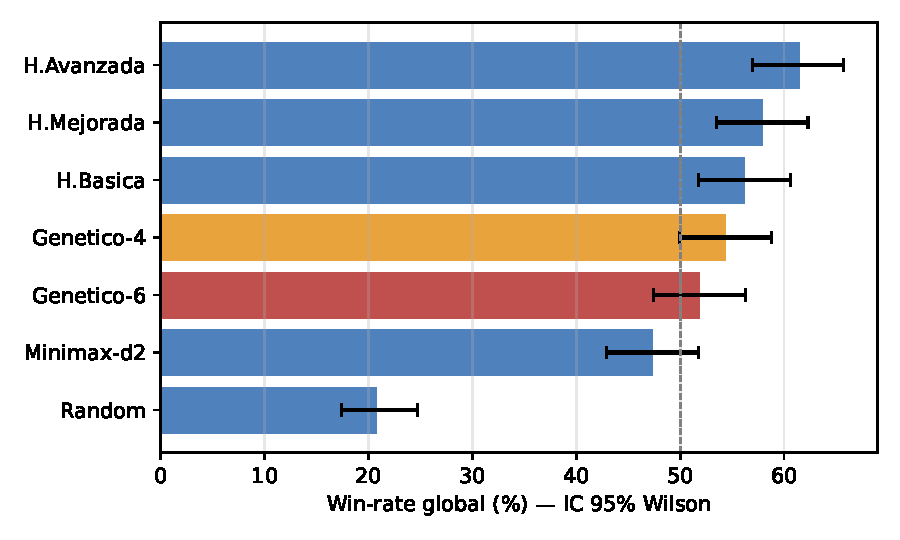
\includegraphics[width=0.95\columnwidth]{figs/figA_torneo.pdf}
\caption{Win-rate global de los siete agentes con IC 95\%. El azar es la línea
base con claridad; la Heurística Avanzada encabeza, y el Genético-6 no supera al
Genético-4.}
\label{fig:torneo}
\end{figure}

\subsection{Experimento B: poda alfa-beta}
\label{sec:poda}
Medimos el coste de búsqueda del minimax por decisión, sobre 40 estados iniciales
aleatorios, contando el número medio de nodos explorados con y sin poda alfa-beta
(Tabla~\ref{tab:poda}, Figura~\ref{fig:poda}). Aprovechamos para medir también el
coste de evaluar las hojas con cuatro frente a seis componentes.

\begin{table}[t]
\centering\small
\resizebox{\columnwidth}{!}{%
\begin{tabular}{ccccc}
\toprule
$d$ & Nodos (poda) & Nodos (sin) & Reducción & ms/dec.\ (4\,/\,6) \\
\midrule
1 & 42.0      & 42.0       & 0.0\%  & 0.7\,/\,1.4 \\
2 & 742.9     & 1\,549.0   & 52.0\% & 10.3\,/\,32.0 \\
3 & 10\,366.3 & 55\,017.7  & 81.2\% & 135.8\,/\,460.7 \\
\bottomrule
\end{tabular}}
\caption{Coste de búsqueda por decisión según la profundidad (promedio sobre 40
estados). La poda no altera la decisión y su ahorro crece con la profundidad
($52\%$ en $d{=}2$, $81\%$ en $d{=}3$). La última columna compara el tiempo por
decisión evaluando las hojas con cuatro vs.\ seis componentes: la evaluación rica
cuesta $\sim 3\times$.}
\label{tab:poda}
\end{table}

\begin{figure}[t]
\centering
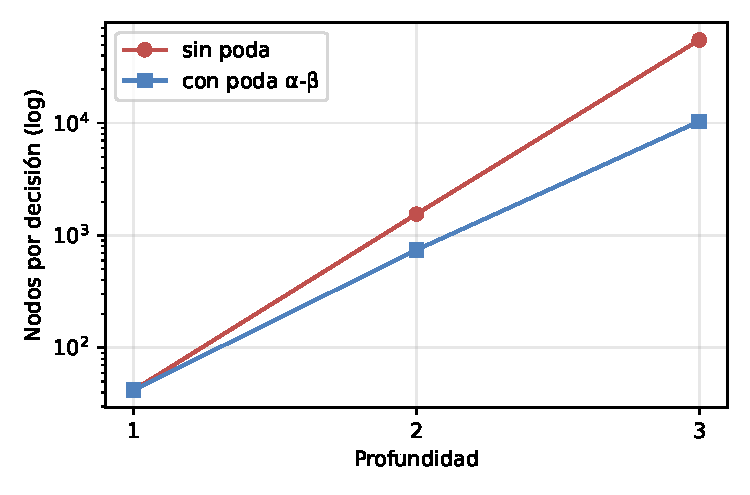
\includegraphics[width=0.8\columnwidth]{figs/figB_poda.pdf}
\caption{Nodos explorados por decisión (escala logarítmica) según la profundidad,
con y sin poda alfa-beta. La poda mantiene exactamente la misma decisión mientras
reduce el trabajo, y la diferencia crece con la profundidad.}
\label{fig:poda}
\end{figure}

\subsection{Experimento C: profundidad y calidad de juego}
\label{sec:profundidad}
¿Mirar más turnos hacia delante mejora el resultado? Medimos la tasa de victorias
del minimax frente a la Heurística Básica a profundidades $d\in\{1,2,3\}$, con 80
batallas por configuración (Tabla~\ref{tab:depthwin}, Figura~\ref{fig:depth}).

\begin{table}[t]
\centering\small
\resizebox{\columnwidth}{!}{%
\begin{tabular}{lccc}
\toprule
 & $d{=}1$ & $d{=}2$ & $d{=}3$ \\
\midrule
Win-rate vs H.\ Básica & 51.2\% & 46.2\% & 42.5\% \\
IC 95\% (Wilson)       & [40.5,\,61.9] & [35.7,\,57.1] & [32.3,\,53.4] \\
Turnos por partida     & 10.2 & 10.8 & 10.4 \\
\bottomrule
\end{tabular}}
\caption{Win-rate del minimax frente a la Heurística Básica según la profundidad
(80 batallas por configuración). Los intervalos de confianza se solapan
ampliamente y abarcan el $50\%$: aumentar la profundidad \emph{no} mejora el
win-rate ---si acaso lo reduce levemente--- en este dominio.}
\label{tab:depthwin}
\end{table}

\begin{figure}[t]
\centering
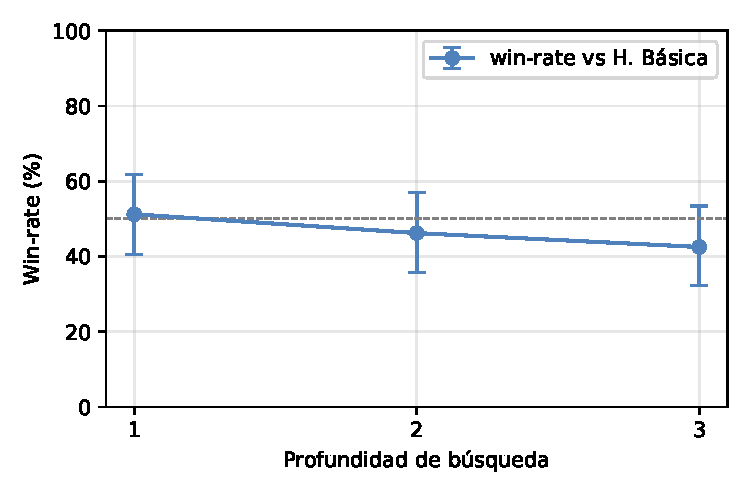
\includegraphics[width=0.8\columnwidth]{figs/figC_profundidad.pdf}
\caption{Win-rate del minimax frente a la Heurística Básica según la profundidad,
con IC 95\%. Más búsqueda no compra más victorias: la tendencia es plana ---incluso
ligeramente descendente--- y los intervalos se solapan con el $50\%$. Lo atribuimos
a la formulación \emph{paranoid} (sobre-defensiva) y a lo cortas que son las
partidas (${\sim}10$ turnos).}
\label{fig:depth}
\end{figure}

\subsection{Experimento D: ¿diversificar el entrenamiento del genético ayuda?}
\label{sec:panel}
Una intuición habitual del aprendizaje automático es que entrenar contra un único
rival \emph{sobreajusta} y que un \emph{panel} de rivales diverso generaliza
mejor. La ponemos a prueba: entrenamos el genético con su \emph{fitness} medido
(a)~contra un solo rival (la Heurística Básica) y (b)~contra un panel (Aleatorio +
Básica + Avanzada), y medimos su win-rate frente a cuatro rivales, incluido
Minimax-$d2$ ---\textbf{no visto} por ninguna de las dos configuraciones. Para que
el resultado no dependa de una semilla afortunada, promediamos \textbf{5 semillas}
independientes (Figura~\ref{fig:panel}). Contra el rival \textbf{no visto}
(Minimax-$d2$) el panel \emph{no} mejora ---de hecho rinde algo peor y con más
varianza ($55.0\pm8.2$ vs.\ $59.7\pm3.2$)--- y globalmente ambos empatan
($55.3\%$ vs.\ $56.9\%$); por rival, las dos configuraciones son indistinguibles.

\begin{figure}[t]
\centering
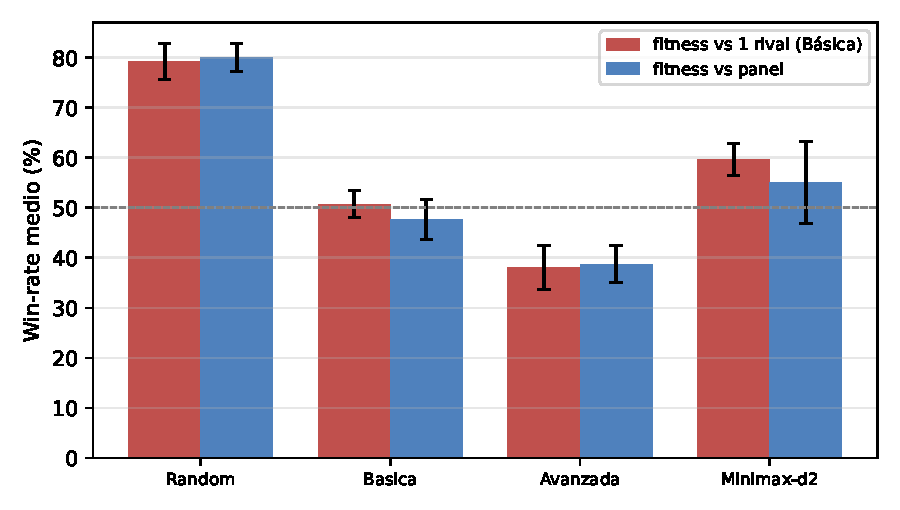
\includegraphics[width=0.95\columnwidth]{figs/figD_panel.pdf}
\caption{Win-rate medio del genético entrenado contra un solo rival vs.\ contra un
panel (5 semillas; barras de error = desviación entre semillas). Contra cada rival
las dos configuraciones son indistinguibles: diversificar el entrenamiento no
aporta ventaja en este dominio.}
\label{fig:panel}
\end{figure}

\paragraph{Un resultado nulo revelador.} Contra la intuición, \textbf{el panel no
generaliza mejor}: las dos configuraciones son estadísticamente indistinguibles
frente a todos los rivales, incluido el no visto. Es un resultado nulo ---pero
informativo---, coherente con el techo estructural del Experimento~E: el combate
es tan simple que todos los genéticos informados convergen cerca de la misma
política, sin importar la diversidad del entrenamiento, de modo que apenas hay
margen para que el sobreajuste se manifieste. (Una corrida aislada puede sugerir
un efecto fuerte por azar; solo el promedio sobre varias semillas lo desmiente
---una lección metodológica en sí misma.)

\subsection{Experimento E: techo de la evaluación}
\label{sec:techo}
El experimento culminante pregunta hasta dónde puede llegar la función de
evaluación, y si una más rica (seis componentes) supera a la de cuatro. Medimos
el win-rate frente al panel (Aleatorio, Básica, Avanzada) en $150$ escenarios
\emph{comunes} a todas las configuraciones (\emph{Common Random Numbers}), a
profundidades $1$ y $2$, para seis vectores de pesos ---por defecto, evolucionado
por el genético y ``solo HP''--- tanto en la evaluación de cuatro componentes como
en la de seis (Tabla~\ref{tab:techo}, Figura~\ref{fig:techo}).

\begin{table}[t]
\centering\small
\begin{tabular}{lcc}
\toprule
Pesos & vs panel ($d{=}1$) & vs panel ($d{=}2$) \\
\midrule
Por defecto (4)           & 54.0          & 54.7 \\
Genético-4 (evolucionado) & 59.3          & 56.0 \\
Solo HP (4)               & \textbf{64.0} & \textbf{64.0} \\
\midrule
Por defecto (6)           & 48.7          & 54.0 \\
Genético-6 (evolucionado) & 54.0          & 51.3 \\
Solo HP (6)               & 46.7          & 49.3 \\
\bottomrule
\end{tabular}
\caption{Techo de la evaluación, cuatro vs.\ seis pesos: win-rate (\%) contra el
panel en $150$ escenarios comunes, a profundidades $1$ y $2$. Ninguna
configuración de seis pesos alcanza el techo de $64\%$ de la de cuatro.}
\label{tab:techo}
\end{table}

\begin{figure}[t]
\centering
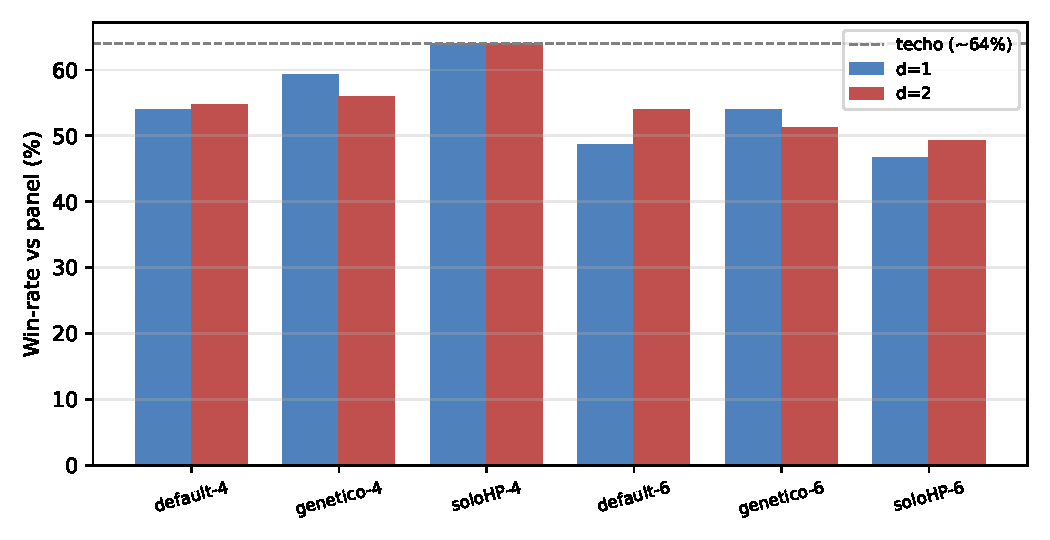
\includegraphics[width=0.95\columnwidth]{figs/figE_techo.pdf}
\caption{Techo de la evaluación: win-rate vs.\ panel de cada configuración de pesos
(cuatro y seis componentes) a $d{=}1$ y $d{=}2$. La línea discontinua marca el
techo ($\sim 64\%$) que solo alcanza ``solo HP'' de cuatro pesos.}
\label{fig:techo}
\end{figure}

\paragraph{Hay un techo, y es de cuatro pesos.} Un vector que pondera \emph{solo}
el HP de equipo alcanza el máximo ($64\%$ a ambas profundidades): el HP acumulado
domina la decisión en este dominio. El genético de cuatro pesos se acerca
($56$--$59\%$) y los pesos por defecto quedan $\sim 10$ puntos por debajo. La
familia de \emph{seis} pesos no llega: su mejor configuración rinde $54\%$, y
``solo HP'' con seis componentes se desploma a $46.7\%$ ---porque su término de HP
pondera un $70\%$ el del Pokémon \emph{activo} (volátil) en lugar del de equipo,
diluyendo justo la señal que más predice la victoria.

\paragraph{Una evaluación más rica no rompe el techo.} A un solo nivel, la
Heurística Mejorada (6 componentes) no mejora a la Avanzada (4): $58\%$ vs.\
$63.3\%$ contra la Básica y $82\%$ vs.\ $87.3\%$ contra el azar, con un empate
técnico en enfrentamiento directo ($45.3\%$, dentro del ruido) y a un coste
$\sim 3\times$ por decisión ($0.40$ vs.\ $0.12$\,ms). Y \emph{dentro} del minimax
con genético tampoco: el Genético-6 no supera al Genético-4 (Experimento~A,
Figura~\ref{fig:torneo}). De hecho, el propio algoritmo genético \textbf{anula} el
componente \emph{peligro de ser noqueado} (peso evolucionado $0.002$): la evolución
``descubre'' que ese componente \emph{duplica} una señal ---la táctica de un
turno--- que el minimax \emph{ya} resuelve al simular el intercambio. El cuello de
botella es, por tanto, la \emph{simplicidad del dominio} (daño dominado por el HP,
sin estados de alteración), no la evaluación ni el optimizador: una buena función
de evaluación debe \emph{complementar} la búsqueda, no \emph{duplicar} la táctica
que el árbol ya calcula.

\section{Resultados y Discusión}

\paragraph{Jerarquía de agentes.} El torneo (Figura~\ref{fig:torneo}) sitúa al
agente aleatorio como el más débil con claridad
($20.8\%$ global, IC $[17.4,24.7]$): cualquier forma de evaluación lo supera. En
el otro extremo, la \textbf{Heurística Avanzada es el mejor agente} ($61.5\%$, IC
$[57.0,65.7]$). El grupo intermedio ---Mejorada ($57.9\%$), Básica ($56.2\%$),
Genético-4 ($54.4\%$), Genético-6 ($51.9\%$) y Minimax-$d2$ ($47.3\%$)--- tiene
intervalos que se solapan en buena medida. Dos lecturas destacan: la búsqueda
(Minimax) no supera a la mejor heurística a un nivel ---lo atribuimos a la
formulación \emph{paranoid} (sobre-defensiva) y a lo cortas que son las partidas
(${\sim}12$ turnos)---, y aunque los pesos evolucionados mejoran al minimax de
pesos por defecto, la evaluación de seis componentes (Genético-6) no aporta sobre
la de cuatro (Genético-4): su enfrentamiento directo es un empate ($50$--$50$).

\paragraph{La búsqueda: la poda paga, la profundidad no.} El resultado más nítido
y robusto está en el coste de búsqueda (Tabla~\ref{tab:poda},
Figura~\ref{fig:poda}): el número de nodos crece de forma explosiva con la
profundidad ($42 \to 743 \to 10\,366$ con poda), y la poda alfa-beta recorta un
$52\%$ de los nodos en $d{=}2$ y un $81\%$ en $d{=}3$, \emph{sin alterar la
decisión} \citep{knuth1975}; el ahorro crece justo donde más se necesita. En
cambio, mirar \emph{más} turnos no compra calidad (Tabla~\ref{tab:depthwin},
Figura~\ref{fig:depth}): el win-rate frente a la Básica no mejora con la
profundidad ---si acaso desciende levemente ($51.2\% \to 46.2\% \to 42.5\%$, con
intervalos que se solapan y abarcan el $50\%$)---, de nuevo por el pesimismo
\emph{paranoid} y la brevedad de las partidas.

\paragraph{El genético optimiza, pero el dominio limita.} El algoritmo genético
mejora con éxito los pesos del minimax (de los manuales a, p.\,ej.,
$(0.26,0.33,0.33,0.08)$, triplicando el peso de la ventaja de tipo). Sin embargo,
diversificar la señal de aptitud \emph{no} ayuda: entrenar el \emph{fitness}
contra un panel de rivales no generaliza mejor al rival no visto que entrenar
contra uno solo (Experimento~D, Figura~\ref{fig:panel}) ---un resultado nulo que
solo se aprecia promediando varias semillas y que es coherente con el límite del
dominio que describimos a continuación.

\paragraph{Un techo estructural del dominio.} El hallazgo de fondo es un
\textbf{techo de $\sim$64\%} frente al panel (Tabla~\ref{tab:techo},
Figura~\ref{fig:techo}): lo alcanza un vector que pondera \emph{solo} el HP de
equipo, y ni los pesos evolucionados ni una evaluación más rica de seis
componentes lo superan ---esta última ni a un solo nivel ni dentro del minimax
con genético (Genético-6). El cuello de botella no es, por
tanto, la función de evaluación ni el optimizador, sino la \emph{simplicidad del
propio combate}: con un daño dominado por el diferencial de HP y sin estados de
alteración, la mejor política es sencilla y todos los agentes informados convergen
cerca de ella. Superar ese techo exigiría enriquecer el \emph{motor}
(p.\,ej.\ estados de alteración), no la evaluación.

\paragraph{Amenazas a la validez.} Pese a usar $80$ batallas por par e intervalos
de confianza, los márgenes siguen siendo de $\pm 5$ puntos, y el daño de
simulación es un \emph{proxy} determinista del combate real estocástico. La
formulación \emph{paranoid} es la limitación de modelado más relevante. El
Experimento~D ilustra además un riesgo metodológico general: una sola corrida
puede sugerir un efecto que desaparece al promediar semillas.

\section{Conclusiones}

Desarrollamos PokeFisi, un simulador de combates Pokémon que integra una familia
de agentes de decisión y permite compararlos de forma reproducible. El modelado
del dominio como un problema de búsqueda adversaria con una función de
evaluación basada en diferenciales acotados resultó suficientemente expresivo
para todos los agentes y, al compartirse entre la heurística avanzada, el
minimax y el genético, facilitó una comparación limpia.

Los experimentos arrojan conclusiones matizadas. El azar es claramente la línea
base; la \emph{Heurística Avanzada} bien calibrada fue el agente más fuerte, por
encima incluso del minimax: su formulación \emph{paranoid} y la corta duración de
las partidas hacen que anticipar turnos aporte poco frente a una buena evaluación
a un nivel ---y, de hecho, aumentar la profundidad no mejora el win-rate. La poda
alfa-beta, en cambio, se reveló inequívocamente útil, reduciendo los nodos
explorados hasta un $81\%$ sin cambiar la decisión y haciendo asequibles las
profundidades mayores.

El algoritmo genético optimizó con éxito los pesos del minimax, pero el dominio
acota lo que ese aprendizaje puede lograr. Diversificar la señal de aptitud
---entrenar contra un panel de rivales en lugar de uno solo--- no mejoró la
generalización (un resultado nulo que solo emerge al promediar varias semillas), y
dejar que el genético optimice una evaluación \emph{más rica} de seis componentes
en lugar de cuatro tampoco ayudó: el Genético-6 quedó por debajo del Genético-4
(Figura~\ref{fig:torneo}) y la propia evolución llegó a anular los componentes
tácticos que la búsqueda ya cubre. Todo apunta a un \textbf{techo estructural}
($\sim$64\%) propio del dominio: con un daño dominado por el HP y sin estados de
alteración, el combate admite una política óptima sencilla a la que todos los
agentes informados se aproximan. La lección es general: una evaluación útil debe
\emph{complementar} a la búsqueda, no \emph{duplicarla}; y superar el techo exige
enriquecer el \emph{motor}, no la evaluación ni el optimizador.

Como trabajo futuro proponemos resolver los nodos como juegos de matriz con
equilibrios de estrategia \emph{mixta} (en lugar de la formulación \emph{paranoid});
usar \emph{auto-juego} coevolutivo para el genético; ampliar los tamaños de muestra
para estrechar los intervalos de confianza; y, sobre todo, enriquecer el modelo con
estados de alteración y mayor estocasticidad ---la vía para superar el techo del
dominio.

% acl.sty ya define \bibliographystyle{acl_natbib}, no hay que repetirlo.
\bibliography{custom}

\end{document}
